%%======================================================================
%% Haupttext
%%======================================================================

\renewcommand{\baselinestretch}{1.2}\normalsize

\chapter{INTRODUCTION}
\label{sec:introduction}

\pagenumbering{arabic}
%\setcounter{page}{2}
\setcounter{footnote}{1}

Write something about IT Service Management, its goals and why software supports achieving these goals. Also describe goals of your project here - why are we doing this? (About one page in sum.)

\chapter{Evaluation of General Characteristics of the Software}

Write a few introductory lines.

\section{Basis facts about the software solution}

Please describe the basic characteristics of the software. Is is a web-based solution? Is it installable or just available as a service? How much effort does the installation take (describe and give a time for the installation)? How old is the software? When did its development start? Which version is it (0.1?)? Is it well established? How many customers are using it? Is it still further developed - are new releases planned and when was the last release? 

Please describe the basic characteristics of the software. 

Is is a web-based solution?

Ja

Is it installable or just available as a service? 

Die Software ist installierbar.



How much effort does the installation take (describe and give a time for the installation)?

Die folgenden Schritte werden auf folgendem Testrechner ausgef�hrt:

Ubuntu 12.04

Es wird die Free Trial Version von Nagios XI heruntergeladen unter:

http://www.nagios.com/products/nagiosxi

Die Trial Version ist eine 60 Tage Testversion von Nagios XI.

Es wird die VMware Virtual Machine (64-bit) Version 2012R1.6 heruntergeladen unter:

http://library.nagios.com/library/products/nagiosxi/downloads/main

Auf der viruellen Maschine l�uft CentOS 6.x und Nagios XI 2012 ist installiert.

Um die VMware Virtual Machine starten zu k�nnen, muss VMware installiert werden.
VMware kann kostenfrei heruntergeladen werden unter:

\url{https://my.vmware.com/web/vmware/free#desktop_end_user_computing/vmware_player/5_0}

Der heruntergeladene VMware-Player wird installiert mit:

sudo sh VMware-Player-5.0.1-894247.x86\_64.bundle

Der VMware-Player wird gestartet und es wird die virtuelle Maschine ausgew�hlt mit 

Open a virtual Maschine.

Die ausgew�hlte virtuelle Maschine wird gestartet mit 

play virtual maschine.

Die virtuelle Maschine wird gestartet. CentOS wird gebootet und Nagios gestartet.

Auf Nagios XI kann jetzt im Browser zugegriffen werde unter:

http://192.168.0.100/

\begin{figure}[htp]
\centering
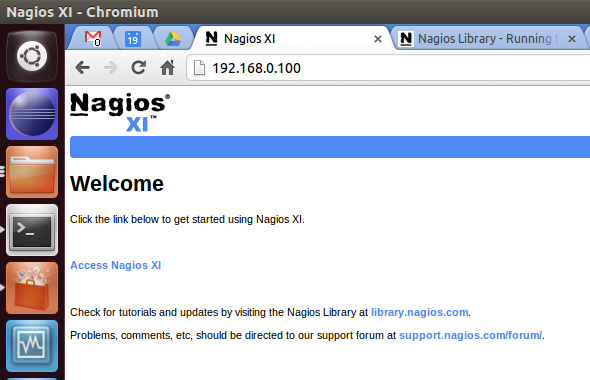
\includegraphics[width=0.6\textwidth]{ingo/bilder/Startseite}
\caption{Startseite von Nagios}
\label{fig:StartseiteVonNagios}
\end{figure}

Das Default Root Passwort ist nagiosxi


How old is the software? When did its development start? 

1999 ver�ffentlichte Ethan Galstad Nagios - dass damals noch NetSaint hie� - als Open Source Projekt.
http://www.nagios.org/about/history

Which version is it (0.1?)? 

Netsaint 0.0.1
\url{http://www.ussrback.com/UNIX/audit/netsaint/index.html}

Is it well established? How many customers are using it? 

Es wird gesch�tzt, dass es weltweit ca 1 Million Nagios Nutzer gibt.
http://www.nagios.org/about/community

Is it still further developed - are new releases planned and when was the last release?

Es wird immernoch weiterentwickelt. Neue Releases sind geplant. Die letzte Version 2012R1.6 ist von 15. Februar 2013.

\section{Versions and price}

Please describe versions, prices and cost models of the software. Is the software open source?
Nagios besteht aus verschiedenen Nagios Projekten:

\begin{itemize}
\item Nagios Core - enth�lt die Core Monitoring Engine und ein basic web interface.
\item Nagios Plugins - er�ffnet die M�glichkeit u.a. Services, Anwendungen und Metriken zu monitoren.
\item Nagios Frontends - erweitert Nagios um zus�tzliche Frontends.
\item Nagios Addons - um Nagios mit Addons zu erweitern.
\item Nagios XI - eine Monitoring- und Alerting-L�sung f�r Unternehmen, bestehend aus Nagios Core und anderen Komponenten.
\end{itemize}

Nagios Core, Nagios Plugins, Nagio Frontends und Nagios Addons sind Open Source.

Das Nagios XI besteht sowohl aus Open Source Software wie dem Nagios Core, als auch aus kommerziellen Lizenzen die nicht unter einer Open Source Software Lizenz ver�ffentlich wurden, wie dem Nagios XI UI und den System Frameworks.

Nagios Core gibt es in verschiedenen Editionen, die sich im Preis, Feature-Set, Suppot und Training unterscheiden.

\begin{tabular}{l|c|c|c|c}
 & DIY & Student & Professional & Business \\
 & Free & \$ 50  & \$ 250 & \$ 1295+ \\
 \hline
Complete Infrastructure Monitoring &	Y&	Y&	Y&	Y \\
Hundreds of Free Addons		&	Y&	Y&	Y&	Y\\
Open Source Monitoring Engine	&	Y&	Y&	Y&	Y\\
Forum Support			&	Y&	Y&	Y&	Y\\
Pre-Configured Virtual Machine	 &	&	Y&	Y&	Y\\
Quickstart Guides	 	&	&	Y&	Y&	Y\\
Web Configuration UI	 	&	&	Y&	Y&	Y\\
Performance Graphing (PNP)	 &	&	Y&	Y&	Y\\
SNMP Trap Support (NSTI)	 &	&	 &	Y&	Y\\
Mobile App	 	 	&	&	&	Y&	Y\\
Business Process Monitoring	 &	&	 &	Y&	Y\\
Custom Maps (Nagvis)	 	&	&	 &	Y&	Y\\
Database Backend	 	 &	&	&	 &	Y\\
Integrated UI	 	 	&	&	&	 &	Y\\
Dashboards	 	 	 &	&	&	&	Y\\
User-Specific Customization	 &	 &	&	 &	Y\\
Configuration Wizards	 	 &	&	&	 &	Y\\
Scheduled Reporting	 	 &	&	&	 &	Y\\
Capacity Planning	 	 &	&	&	 &	Y\\
Executive Reports	 	 &	&	&	 &	Y\\
Bulk Management	 	 	 &	&	&	&	Y\\
Configuration Rollback	 	 &	&	&	 &	Y\\
Audit Logging	 	 	 &	&	&	&	Y\\
Executive Reports	 	 &	 &	&	&	Y\\
Email and Phone Support	 	 &	 &	&	&	Y\\
\end{tabular}

Nagios XI ist eine Monitoring und Alerting-L�sung f�r Unternehmen, die auf Nagios Core aufbaut. Nagios besitzt ein PHP Web Interface, eine integrierte Performance Visualisierung, anpassbare Dashboards, eine Web Configuration GUI, Configuration Wizards, User Management und vieles mehr.

Vergleich von Nagios Core und Nagios XI:

\begin{tabular}{l|c|c}
Feature & Nagios XI & Nagios Core OSS \\
\hline
\textbf{Infrastructure Monitoring}	&  &  \\
-Servers				&Y  &Y  \\
-Network Elements		&Y  &Y  \\
-Applications			&Y  &Y  \\
-System Metrics			&Y  &Y  \\
-Custom Services			&Y  &Y  \\
\textbf{Alerting}			&  &  \\
-Email				&Y  &Y  \\
-Mobile Phone			&Y  &Y  \\
-Custom Method			&Y  &Y  \\
\textbf{Reports}				&Y  &Y  \\
\textbf{User-Specific Interface Customization}	&Y  &  \\
\textbf{Advanced Dashboards}		&Y  &  \\
\textbf{Web Configuration Interface}	&Y  &  \\
\textbf{Configuration Wizards}		&Y  &  \\
\textbf{Session Authentication}		&Y  &  \\
\textbf{Performance Graphs}		&Y  &  \\
\textbf{Database Backend}		&Y  &  \\
\textbf{Multi-Tenant Capabilities}	&Y  &Y  \\
\textbf{Customizable}			&Y  &Y  \\
\textbf{Distributed Monitoring Capabilities}	&Y  &Y  \\
\textbf{Extendable Architecture}		&Y  &Y  \\
\textbf{Proven OSS Core}			&Y  &Y  \\
\textbf{Professional Support Options}	&Y  &Y  \\
\end{tabular}

Unter

\url{http://www.nagios.com/products/nagiosxi/pricing/}

sind die Preise f�r die jeweiligen Lizenzen f�r Nagios XI aufgef�hrt.

Die Preise f�r Nagios XI h�ngen vom Lizenz Level ab, dass gew�hlt wird. Die Lizenzlevel h�ngen von der Anzahl der unterst�tzten Hosts ab:

\begin{tabular}{l|l|l|l}\label{LizenzLevel}
License Level	& Initial Price	 & Renewal Price	& Support Incidents Included \\
\hline
Unlimited Hosts	& \$4,995 USD	&\$4,000 USD		& 10 \\
101 - 200 Hosts	& \$2,995 USD	&\$2,000 USD		& 5 \\
UP To 100 Hosts	& \$1,995 USD	&\$1,650 USD		& 3 \\
\end{tabular}

Nagios XI 2012 ist in zwei Editionen verf�gbar: Standard und Enterprise.

\begin{tabular}{p{3cm}|p{1cm}|p{1cm}|p{10cm}}
Features \ Edition & Stan\-dard & Enter\-prise & Benefit \\
\hline
Configuration Rollback & Y & Y & Allows administrators to easily recover from configuration errors by rolling back to known good snapshots. \\

New wizards and components &Y&Y& New wizards and components add additional functionality and are automatically installed and upgraded with each new release.\\

Tools menu &Y&Y& Allows users to integrate custom and 3rd-party applications directly into the XI interface to increase productivity.\\

Bandwidth report &Y&Y& Provides detailed daily, monthly, quarterly, and yearly bandwidth reports for routers and switches.\\

Executive summary report &Y&Y& Provides management, administrators, and decision-makers with at-a-glance visibility into recent alerts and activity.\\

Heartbeat monitoring &Y&Y& Provides essential monitoring of critical hosts and applications on remote machines.\\

Custom action URLs &Y&Y& Provides users with ability to add customized links to each host and service.\\

NOC screens &Y&Y& Provides at-a-glance overview of IT operations from a single screen.\\

Host rename tool &Y&Y& Allows administrators to quickly and efficiently rename hosts and retain historical performance and alert data.\\

Emailed reports &Y&Y& Allows users to quickly email reports to themselves, team members, and other decision makers.\\

Enhanced Configuration GUI &Y&Y& Improved GUI for monitoring configuration makes complex tasks easier.\\

Mobile Interface &Y&Y& Provides compact, intuitive interface for mobile phones and devices.\\

Custom Host and Service Actions &Y&Y& Allows administrators to define commands and actions that are readily available to user for troubleshooting and fixing problems, opening trouble tickets, and more.\\

Capacity planning report &&Y& Provides trending analysis and capacity planning for predicting future upgrade requirements.\\

Web-based server console access &&Y& Provides fast, web-based access to the XI server console for performing upgrades and maintenance.\\

Advanced business process monitoring &&Y& Provides advanced reporting of critical business processes with automatic group synchronization, advanced grouping logic, and advanced permissions.\\

Scheduled reports &&Y& Provides regularly scheduled reports to be sent to decision makers, management, and administrators via email.\\
\end{tabular}

\begin{tabular}{p{3cm}|p{1cm}|p{1cm}|p{10cm}}
Features \ Edition & Stan\-dard & Enter\-prise & Benefit \\
\hline

Scheduled pages &&Y& Allows users to schedule any XI web page to be delivered via email as PDF attachments on a scheduled basis. Great for sending dashboards, custom screens, and more.\\

Bulk modification tool &&Y& Allows administrators to quickly modify attributes of thousands of hosts and services in a few simple steps.\\

Bulk notification settings tool &&Y& Allows administrators to quickly deploy notification settings to users in a few simple steps.\\

Audit Logging &&Y& Provides an audit trail of changes and modifications to ensure policy compliance.\\

Improved Autodiscovery &&Y& Provides easy integration with bulk monitoring wizard for rapid monitoring of newly discovered devices.\\

Remote Machine Monitoring &&Y& Provides easy to use monitoring of remote machines and devices on external networks without firewall modifications.\\

Escalation Wizard &&Y& Allows users to easily create notification escalation policies.\\

\end{tabular}

Die Kosten f�r die Enterprise Edition werden auf den Basis-Kaufpreis addiert:

\begin{tabular}{l|l}
 Initial Price	& Renewal Price \\
\$1,500 USD	& \$750 USD \\
\end{tabular}

Es gibt auch eine kostenlose Lizenz von Nagios XI f�r kleine Umgebungen:
Mit der kostenlosen Lizenz lassen sich bis zu 7 Hosts/Nodes mit einer unbegrenzten Anzahl von Services monitoren. In der freien Lizenz sind keine Support Dienste enthalten.

Pro Nagios XI Lizenz kann ein Monitoring Server betrieben werden.
Werden mehrere Monitoring Server ben�tigt, k�nnen mehrere Nagios XI Lizenzen erworben werden. Dabei gelten folgende Preisnachl�sse:

\begin{tabular}{l|l}
Licenses &	Discount \\
\hline
2 - 4 & 10\% \\
$>5$   & 20\% \\
\end{tabular}

Nagios XI wird in verschiedenen Formaten zum Download angeboten:

\begin{itemize}
\item Als VMware Virtual Maschine 32-bit und 64-bit: eine VMware virtual machine auf der CentOS 6.x l�uft und auf der Nagios XI 2012 installiert ist.

\item Als vSphere OVF Template 32-bit und 64-bit: ein OVF template auf dem CentOS 6.x l�uft und Nagios XI 2012 installiert ist.

\item Als Microsoft Virtual Machine 32-bit und 64-bit: eine Microsoft Virtual Machine auf der CentOS 6.x l�uft und auf der Nagios XI 2012 installiert ist.

\item Als Linux Source Installer: um Nagios XI 2012 manuell zu installieren.
\end{itemize}

\section{Usability}

Does the user interface and layout look up to date? Is it easy to understand and learn the functionalities of the software? Is the user interface efficient? Are the functionalities intuitive? Is the choice of the colors reasonable? Please answer the questions and grade the usability of the software - 5-extraordinary good - 1-very poor.

\section{Performance}

Describe if the performance of the software. Is it satisfying? Are the response times in order? Are there any performance critical operations? Please answer the questions and evaluate the performance between 5-extraordinary good and 1-the screen war frozen with the first klick :)

\section{Documentation}

Describe how well the software is documented on a scale between 5-extraordinary well to 1-no documentation available. Please also describe which tutorials, seminars or certification courses are available. 
\section{Support}

How is the software supported? Is there a number to call, a web form/ email address, a forum (and if so, how are the replies - fast and well explaining?)? Does the support have to be payed? Try to ask the support a question and report the reaction. If you got a reply - was the reply competent? Evaluate the support between 5-extraordinary good to 1-no support.

Mit einer Nagios XI Lizenz gibt es 

\begin{itemize}
 \item technischen Support - via EMail oder in einem speziellen customer-only Abschnitt im online forum unter

\url{http://support.nagios.com/forum}

\item Support - je nach Lizenz-Level werden pro Jahr bis zu 10 Support Incidents bearbeitet.

\item Training - ein volles Jahr Zugriff auf Ressourcen f�r das Selbststudium von Nagios XI und Nagios addons.

\item eine unbefristete Lizenz - die Lizenz der Software ist dauerhaft, selbst wenn kein zuk�nftiger Support oder Wartungsvertr�ge geschlossen werden.

\item die Nagios Library - f�r ein volles Jahr kann auf spezielle Nagios Libraries zugegriffen werden, mit customer-only Tutorials, Videos und Tech Tipps.

\item Produkt-Einfluss - Feature Requests k�nnen eingereicht werden.

\item freie Lizenzwahl f�r selbstgeschriebene Erweiterungen - es k�nnen beliebige Lizenzen f�r eigene Erweiterungen f�r Nagios XI gew�hlt werden: z.B. open source, propriet�r oder public domain.
\end{itemize}


\section{Errors and Bugs}

Describe errors and bugs of the software which you found during testing.

\chapter{Evaluation of the ITSM Specific Functionalities}

\section{ITSM Processes}
\label{sec:itsmprocesses}

Describe the support of the processes with a number from 1-5 (5 for fully supported), describe also "what" it supported and "what not". Use our scribe notes with detailed information about the processes to have an idea about what could be supported. Give further descriptions "how" it is supported and about the usability of the process features in the column "comments". Describe as many details as possible.

\begin{table}[h!]
\caption{Supported ITSM Processes}
\vspace*{0.3cm}
\begin{tabular}{|p{6.1cm}|p{4.5cm}|p{4.5cm}|}\hline
\textbf{ITSM Process}             &\textbf{Supported (1-5)}        &\textbf{Comments}\\\hline\hline
\textbf{Service Strategy}          &                                &\\
Strategy Generation            &                                &\\
Demand Management                   &                                &\\
Service Portfolio Mgmt.                   &                                &\\
Financial Management                   &                                &\\\hline
\textbf{Service Design}          &                                &\\
Service Catalogue Mgmt.                   &                                &\\
Service Level Management                   &                                &\\
Capacity Management                   &                                &\\
Availability Management                   &                                &\\
IT Service Continuity Mgmt.                   &                                &\\
Information Security Mgmt.                   &                                &\\
Supplier Management                   &                                &\\\hline
\textbf{Service Transition}          &                                &\\
Transition Planning and Support                   &                                &\\
Change Management                   &                                &\\
Service Asset and Configuration Mgmt.                   &                                &\\
Release and Deployment Mgmt.                   &                                &\\
Service Validation and Testing                   &                                &\\
Evaluation                   &                                &\\
Knowledge Management                   &                                &\\\hline
\textbf{Service Operation}          &                                &\\
Event Management                   &                                &\\
Incident Management                   &                                &\\
Request Management                   &                                &\\
Problem Management                   &                                &\\
Access Management                   &                                &\\\hline
\textbf{Continual Service Improvement}          &                                &\\
7-Step Improvement                   &                                &\\
Service Reporting                   &                                &\\
Service Measurement                 &                                &\\\hline
\textbf{General}                   &                                 &\\
Service Desk                       &                                 &\\
Raci Authority Matrix                    &                           &\\\hline
\end{tabular}
\label{tab:SupportedITSMProcesses}
\end{table}

\section{IT Service Management Roles}
\label{sec:ITSMRoles}

Described the support of the ITSM roles individually.

\section{Scenarios}
\label{sec:scenarios}

\subsection{Design of an Email Service}
\label{sec:emailServiceDesign}

Design an email service as a new service within the service management software which has to be evaluated. Please consider if supported:
\begin{itemize}
\item Creating and formalizing a \emph{Service Design Package} (SDP)
\item Creating and formalizing \emph{Service Acceptance Criteria} (SAC)
\item Creating and formalizing \emph{Service Level Requirements} (SLR) which develop to the \emph{Service Level Agreement} (SLA) within the design process.
\end{itemize}

Lookup all necessary information about the documents in your scribe notes. Are measurable goals for the services supported by the software? How about SLA-Monitoring (SLAM) and Service Improvement Plans? Are different service levels for the same service supported? Are different SLA types supported (service-based, customer based, multi-level)?

Describe how your software supports this procedure. Use also screen shots to visualize that.

\subsection{ITIL Roles}
\label{sec:itilRoles}

Check which of the ITIL roles (\url{http://wiki.en.it-processmaps.com/index.php/Roles_within_ITIL_V3}) are supported by your software or how it is possible to define ITIL roles for your service. Then establish as many ITIL roles as possible in your test system.

\subsection{Service Catalogue}
\label{sec:serviceCatalogue}

Check if the life cycle phases \emph{Service Pipeline}, \emph{Service Catalogue} and \emph{Retired Services} are supported by your software. Add the new Email Service as new service to the service pipeline, then transfer it to the service catalogue and finally retire the service. Is it possible to get information about all services in the life cycle? If yes describe how that works. Which information are available for each service? Is there a division in \emph{business service catalogue} and \emph{technical service catalogue}?

Describe how your software supports this procedure. Use also screen shots to visualize that.

\subsection{Further Management of the Email Service}
\label{sec:furtherManagement}

Note that you need to preserve capacities for your email service. Is there a capacity management information system? If yes then develop a capacity plan and  reserve capacities for your email service. How about planning of personnel resources?

Also develop an availability plan for your email service if this is supported by the software. Is the ITIL role of the Availability Manager supported?

Is it supported by the software to plan capacities and availability in an alternating way?

How about a continuity plan for your Email service - is it possible to establish that in the software? Develop an exemplary continuity plan for the email service.

How is information security management and supplier management supported. If supplier management is supported, add exemplary suppliers with underpinning contracts for basis functionality of your email service - e.g. use cloud services to store the emails or your service. Safe the contract in the supplier and contract data base if available (SCD - Supplier and Contract Database).

\subsection{Configuration Management}
\label{sec:configurationManagement}

Add all necessary configuration items to implement your email service as configuration items in the Configuration Management Database (CMDB) of the system. Note that it is normal to have thousands if not millions of configuration items within the system. This is of course not the case in our test system but consider adding different CI-types as necessary infrastructure and servers, routers, documents, chairs, IP-adresses, other hardware and services, buildings, persons, etc. Add for each of the items a configuration record with all describing information. Are agents supported, which write infrastructure automatically in the CMDB? Is a CMS available to host the CMDB?

\subsection{Change Management}
\label{sec:changeManagement}

Simulate all three types of changes which you know from the lecture. Rise a RFC (request for change) first. Then initiate a normal change to your service, e.g. migrating the email service to a new server. Also increase the storage capacity of your email service from the initial value of $x$ MB to $y$ MB. Since this change is not very risky, establish it as \emph{standard change}. Define the CAB (Change Advisory Board) and a ECAB (Emergency Change Advisory Board). Simulate the situation that your email system got hacked - how is the handling of that situation supported by your software?

Now think about developing your email service further, e.g. by adding IMAP or POP or by adding a web interface. Plan those changes in a \emph{Forward Schedule of Changes} (FSC) if available. Are the 7Rs supported somehow to make sure that the right questions are asked before the change is realized?

\subsection{Definite Media Library}
\label{sec:definiteMediaLibrary}

Is there a \emph{Definite Media Library} (DML) to represent media CIs in different versions? All media items should also be available as CI in the CMDB. Think about which software you need to realize your email service and create configuration items with Master copies of this software which are also represented in the DML.

\subsection{Knowledge Management}
\label{sec:knowledgeManagement}

Consider to safe further information about your email service, as current users, status information about the service utilization, down times, etc. Safe those information to the \emph{Service Knowledge Management System} (SKMS) if possible. Is it supported to safe status information about the service automatically?

\subsection{Event, Incident and Problem Management}
\label{sec:eventIncidentProblemManagement}

Since we did not consider Service Operation in the lecture so far, we need to have a brief introduction. Note that events can be any change of status - informative events where no action is required, hitting some predefined level for some parameter, exceptions that some resource or service is not in operation as usual. Incidents are events which interrupt or potentially interrupt a service. Events which are incidents have to be reported using an interface of the \emph{Event Management System} to the \emph{Incident Management}. Also the breakdown of an configuration item which has no direct impact for a service is an incident. Note that incidents need to be treated and prioritized according to \emph{impact} and \emph{urgency}. Then, a problem is a not known cause for one or several incidents. There are \emph{problem records} with the complete history of a problem and also a \emph{Known Error Data Base} (KEDB) with all of these known errors and their records.

The single point of access for the customer is always the \emph{service desk}. Each call of a customer is an incident.

Consider different events, incidents and problems for your email service and check how they can be formally treated with your software system. How is the work of the service desk supported? Treat events, incidents and problems based on a few examples. 

\chapter{Conclusion}

Conclude your evaluation with some overall statements (about 1/2 page).